

\chapter{Fourier Transform}

\section{Introduction}

This chapter include simulation about spectral analysis using tools such as Discrete Fourier Transfrom (DFT) \nomenclature{DFT}{Discrete Fourier Transfrom} and Fast Fourier Transform (FFT) \nomenclature{FFT}{Fast Fourier Transform}.

\section{Reminder}

\subsection{Fourier Transform Relation}

\underline{Notation:} taken from chapter 4 in \cite{DSP_DimitrisManolakis}

\begin{table}[!h]
	\centering
\begin{tabular}{|c|c|c|} \hline

Time: Continuous or Discrete & Analysis (Frequency Domain) & Synthesis (Time Domain) \\ \hline
CTFS & $c_k \, = \, \displaystyle\frac{1}{T_0} \displaystyle\int_{T_0} x(t) \, e^{-j  \, k \, 2 \pi f_0 t} dt$ 	& $x(t) \, = \, \displaystyle\sum_{k \, = \, - \infty}^{+ \infty} c_k \, e^{j \, k \, 2 \pi F_0 \, t}$   \\ \hline
CTFT & $X(F) \, = \, \displaystyle\int_{-\infty}^\infty x(t) \, e^{-j 2\pi F t} dt $	& $x(t) \, = \, \displaystyle\int_{-\infty}^\infty X(F) \, e^{j 2\pi F t} dF $ \\ \hline
DTFS    & $c_k \, = \, \displaystyle\frac{1}{N} \displaystyle\sum_{n \, = \, 0}^{N \, - \, 1} x[n] \, e^{-j  \, \frac{2 \pi}{N} \, k \,n} $ & $x[n] \, = \, \displaystyle\sum_{k \, = \, 0}^{N \, - \, 1} c_k \, e^{j  \, \frac{2 \pi}{N} \, k \,n}$ \\ \hline
DTFT    & $X(\omega) \, = \, \displaystyle\frac{1}{N} \displaystyle\sum_{n \, = \, - \infty}^{\infty} x[n] \, e^{-j  \, \omega \,n} $ & $x[n] \, = \, \displaystyle\int_{2 \pi} X(\omega) \, e^{j  \, \omega \,n} d \omega$ \\ \hline
\end{tabular}
\caption{Fourier Formula}
\label{Tb:Fourier_Processing:Fourier_Relation}
\end{table} 


\newpage
\subsection{Frequency Variables}

\begin{itemize}

\item Relation between \textit{continous frequency} $F$ [Hz] and \textit{continous angluar frequency} $\Omega$ [rad/s]:

\begin{equation}
\Omega \, = \, 2 \pi \, F
\label{eq:Omega_Fs}
\end{equation}

\item Relation between \textit{normalized angular frequency} $\omega$ [rad/cycle] and \textit{continuous angular frequency} $\Omega$ [rad/s] \cite{DSP_DimitrisManolakis}
    
\begin{equation}
    \omega  = \displaystyle\frac{\Omega}{F} 
\end{equation}

\item Moving between Hz $\leftrightarrow$ [rad/cycle]

\begin{table}[!h]
	\centering
\begin{tabular}{|c|c|} \hline
radian/cycle $\rightarrow$  Hz & Hz $\rightarrow$ radian/cycle \\ \hline 
 $ F \, [\text{Hz}] \, = \, \omega [\text{radian/cycle}] \, \times \, \left( \, \displaystyle\frac{F_s}{2 \pi} \, \, \right)$ & $\omega \, [\text{radian/cycle}] \, = \, F [\text{Hz}] \, \times \, \left( \, \displaystyle\frac{2 \pi}{F_s} \, \right)$ \\ \hline
\end{tabular}
\caption{Fourier Formula}
\label{Tb:Fourier_Processing:frequency_variables}
\end{table} 

\item Diagram illustration of \autoref{Tb:Fourier_Processing:frequency_variables}\cite{DSP_DimitrisManolakis}



\begin{figure}[h]
\centering
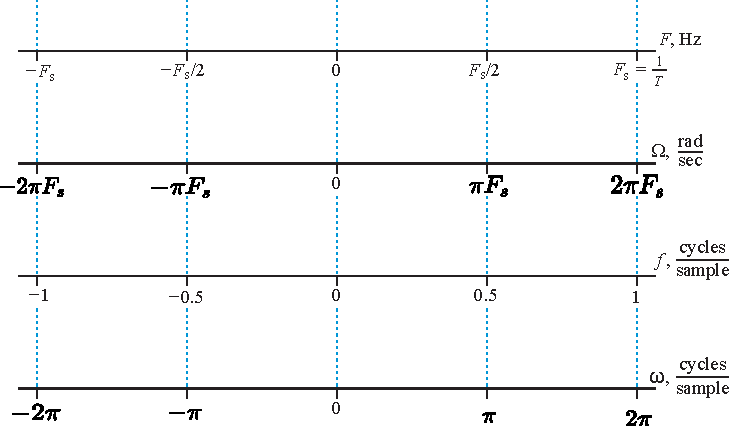
\includegraphics[scale = 1.2]{Figures/Fourier_Summary/frequency_variables}
\label{fig:Fourier_Summary:frequency_variables}
\caption{Frequency Variables illustration of \autoref{Tb:Fourier_Processing:frequency_variables}\cite{DSP_DimitrisManolakis}}
\end{figure}

\end{itemize}


\newpage
\subsection{DTFT-CTFT Relation}


See \cite{signal_processing_Lathi}.

\begin{equation}
\begin{array}{lll}
X_{\delta}(F) \, &=& \, \displaystyle\frac{1}{T_s} \displaystyle\sum\limits_{k \, = \, -\infty}^{+ \infty} X_c \left(\, F \, - \, k \,F_s  \,\right) \\ \\
                &=& \, X(\omega)
\end{array}
\label{Eq:DTFT-CTFT-Relation}
\end{equation}

\begin{itemize}
    \item $X(\omega)$ is an DTFT of $x[n] \leftrightarrow$ DTFT of a discrete signal
    
    \item $X_c(F)$: CTFT of the $x(t) \leftrightarrow$ CTFT of a analog continous signal
    
    \item $X_{\delta}(F)$: CTFT of $x(n \, T_s) \leftrightarrow$ CTFT of a sampled signal 
    
\end{itemize}

\autoref{Eq:DTFT-CTFT-Relation} states that DTFT and CTFT of a sampled signal are the same, and if we want to retrieve the CTFT of $x(t)$, we need to multiply by $T_s$

\todo{DTFT-CTFT Relation}: \textit{to insert a figure for \autoref{Eq:DTFT-CTFT-Relation}}.


\subsection{Fourier Transform Table}

\begin{table}[!h]
	\centering
\begin{tabular}{|c|c|} \hline
$x(t)$  & $X(F)$ \\ \hline 
$\Pi\displaystyle \left( \, \frac{t}{\tau} \,\right)$ & $\text{sinc} (\pi \, F \, \tau)$ \\ \hline
$2\, B \, \text{sinc}(2 \pi \, B \, t)$ & $\Pi\displaystyle \left( \, \frac{F}{2 \, B} \,\right) $\\ \hline
$\Delta\displaystyle \left( \, \frac{t}{\tau} \,\right)$ & $ \displaystyle\frac{\tau}{2} \, \text{sinc}^2 \left( \displaystyle\frac{\pi \, F \, \tau}{2}   \right)$ \\ \hline
$ B \, \text{sinc}(\pi \, B \, t)$ & $\Delta\displaystyle \left( \, \frac{F}{2 \, B} \,\right) $\\ \hline
 $\displaystyle\sum_{n \, = \, - \infty}^\infty \delta(t \, - \, n \, T_0)$ & $ f_0 \, \displaystyle\sum_{n \, = \, - \infty}^\infty \delta(F \, - \, n \, f_0)$ \\ \hline
\end{tabular}
\caption{CTFT Transform Pair}
\label{Tb:Fourier_Processing:CTFT_Table}
\end{table} 

\newpage
\section{Analog Signal}

\underline{Source:} see example 5.8 in \cite{signal_processing_Lathi},\\

The continuous time domain signal to be taken is a decaying exponential:

\begin{equation}
x(t) \, = \, \text{exp}(-0.5 \, t) \, u(t) \leftrightarrow \, X(\Omega) \, = \, \displaystyle\frac{1}{j \, \Omega \, + \, 0.5}
\label{eq:inf_time_freq}
\end{equation}

Signal of \autoref{eq:inf_time_freq} is infinite both in time and frequency domain.

$\mathrm{1}^\mathrm{st}$ step is to do an approximation in frequency domain, that is choosing the maximum frequency $B$. Once we have $B$, we can apply Nyquiste theorem to have an appropriate $F_s$ and hence a $T_s$, so we can truncate in time and obtain suitable number of samples.


\subsection{Truncation in frequency domain}

\begin{itemize}
    
\item Spectrum is infinite in frequency domain:    
    
Infinite in frequency domain means no maximum frequency to be taken to apply Nyquist sampling theorem $\rightarrow$ need to \tbi{truncate in frequency so we can choose a sampling frequency} $F_s$.\\

\item As a criteria to truncation: what is the value of $\Omega$ at which the frequency content is bellow 2 \% ? 

In other words, this $\Omega$ captures 98 \% of the frequency content of the signal.

\item \underline{Computations:} 

\begin{itemize}

\item $ \displaystyle\left\lvert X(\Omega) \displaystyle\right\rvert \, = \, \displaystyle\frac{1}{\sqrt{ \Omega^2\, + \, 0.5^2} } \, = \, 2 \, \times \, 0.01 \, = \, 0.02 $ 

\item Solving for $\Omega$ we get: $\Omega \, = \, 50 \text{ rad/s}$

\item Using \autoref{eq:Omega_Fs}: $B \, = \, \displaystyle\frac{\Omega}{2 \, \pi} \, = \, \displaystyle\frac{50}{2 \, \pi} \, = \displaystyle\frac{25}{\pi}$ Hz

\end{itemize}

\item The maximum frequency is $\displaystyle\frac{25}{\pi}$ Hz.

Applying Nyquiste states that $F_{s_{\text{min}}} \, = \, 2 \, B \, = \, 2 \, \times \, \displaystyle\frac{25}{\pi} \, = \, \displaystyle\frac{50}{\pi}$ Hz

\item Having $F_{s_{\text{min}}} \, = \, \displaystyle\frac{50}{\pi}$ gives a minimum sampling period $T_{s_{\text{min}}} \, = \, \displaystyle\frac{\pi}{50} $ s

\end{itemize}

So as summary, from frequncy truncation we get:

\begin{itemize}

\item $B \, = \, \displaystyle\frac{25}{\pi} \, \approx \, 8$ Hz

	\begin{itemize}
	\item This $B$ captures 98 \% of the frequency content of the signal
	\end{itemize}

\item $F_{s_{\text{min}}} \, = \, \displaystyle\frac{50}{\pi}$ Hz

\end{itemize}
  

\subsection{Truncation in time domain}

\begin{itemize}
    
\item Waveform in infinite in time domain:

After we solve for $T_s \, = \, \displaystyle\frac{\pi}{50}$ s, there is another question to be asked: for \tbi{how long do we need to sample} ? $\leftrightarrow$ This signal is going forever, we can't just keep sampling forever\\


So we need to solve for \tbi{sampling duration} $T_0 \, \leftrightarrow$  signal duration

\item \underline{Criteria to solve the problem:} We know that the signal is a decaying exponential, we can see for some value of $T_0$ where the  \tbi{amplitude value of the signal} $x(t)$  \tbi{is very low}, and by this we are \tbi{not throwing some high value amplitude (information)}.\\

\item Computing: 
	
	\begin{itemize}
	\item We try for example for $T_0 \, = \, 16$ s, we get $x(16) \, = \, e^{-0.5 \, (16)} = \, e^{-8} \, = \, 3.3 \, e^{-4}$, very small number
	
	\item If we choose $T_0 \, = \, 16$, the number of sample we get in this period using a sampling rate $T_s \, = \, \displaystyle\frac{\pi}{50}$ is: $N_0 \, = \, \displaystyle\frac{T_0}{T_s} \, = \, 254.65$
	
	
	\item However, the number of samples we need to grab need to be integer, so let's say we need to grab 256 samples
	
	\item We resolve again for $T_s$ using $N_0 \, = \, 256$ samples, and we get $T_s \, = \, \displaystyle\frac{1}{16}$ seconds 
\end{itemize}

\end{itemize}

The rest is done via programming part.\\

\subsection{Results}

\begin{figure}[h]
\centering
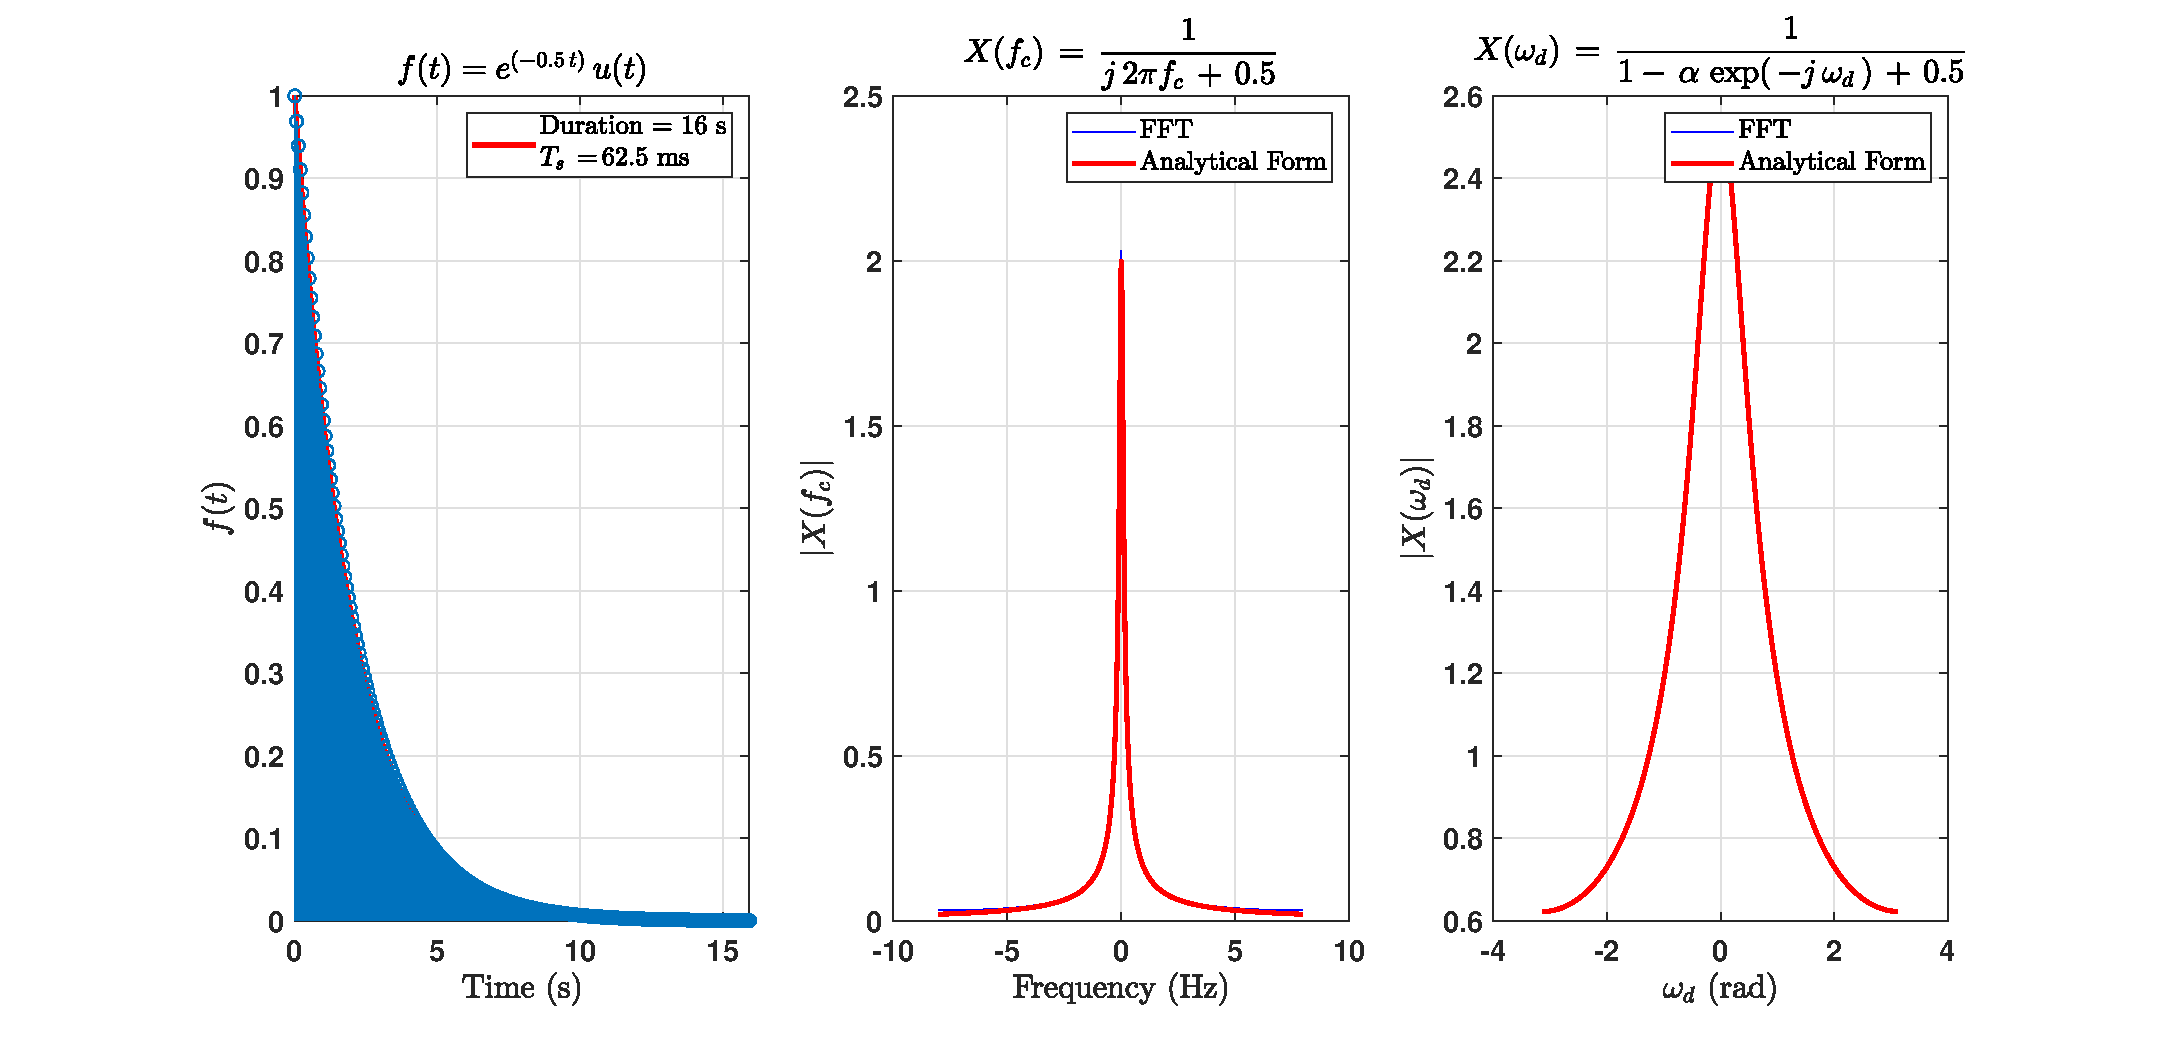
\includegraphics[scale = 0.5]{Figures/Sim_Fourier_Transform/CTFT_DTFT_using_fft_fs_16.eps}
\label{fig:Sim_Fourier_Transform:CTFT_DTFT_using_fft_fs_16}
\caption{Base line: Signal Duration is 16 s and $F_s \, = \,$ 16 Hz}
\end{figure}



\newpage
\subsection{Summary}

As a \tbi{summary} we have:

\begin{itemize}

\item $\mathrm{1}^\mathrm{st}$ question we ask since the signal $x(t)$ isn't band limited $\leftrightarrow$ keep going forever in frequency domain: \tbi{how do we choose the sampling rate (sampling period)} $F_s \, (T_s)$

	\begin{itemize}
	\item what is a suitable criteria to choose some maximum frequency to represent the bandwidth $B$ of the signal ?
	
	\item Once we choose $B$, we apply Nyquiste to have a minimum sampling frequency $F_{s_{\text{min}}}$
	\end{itemize}
	
\item $\mathrm{2}^\mathrm{nd}$ question: for \tbi{how long we keep sampling $\leftrightarrow$ (signal truncation)} ?

	\begin{itemize}
	\item choose some value of $T_0$ in which values (content) of the signal is preseverd
	
	\end{itemize}

\item Always recall that:
	
\begin{equation}
\overbrace{N}^{\text{nb of samples}} \, = \, \displaystyle\frac{\overbrace{T_0}^{\text{Signal duration}}}{\underbrace{T_s}_{\text{Sampling Period}}} \, \in \,\mathbb{N}
\end{equation}
	

\end{itemize}


\newpage
\section{Working with fft}

Now we turn attention to the usage of \verb|fft| command to compute the spectrum.\\

In \autoref{fig:Sim_Fourier_Transform:sinc2_B_10Hz_Fs_30Hz}, we have the result of $x(t) \, = \, B \, \text{sinc}(\pi \, B \, t) \leftrightarrow \, \Delta\displaystyle \left( \, \frac{F}{2 \, B} \,\right) $

\begin{figure}[h]
\centering
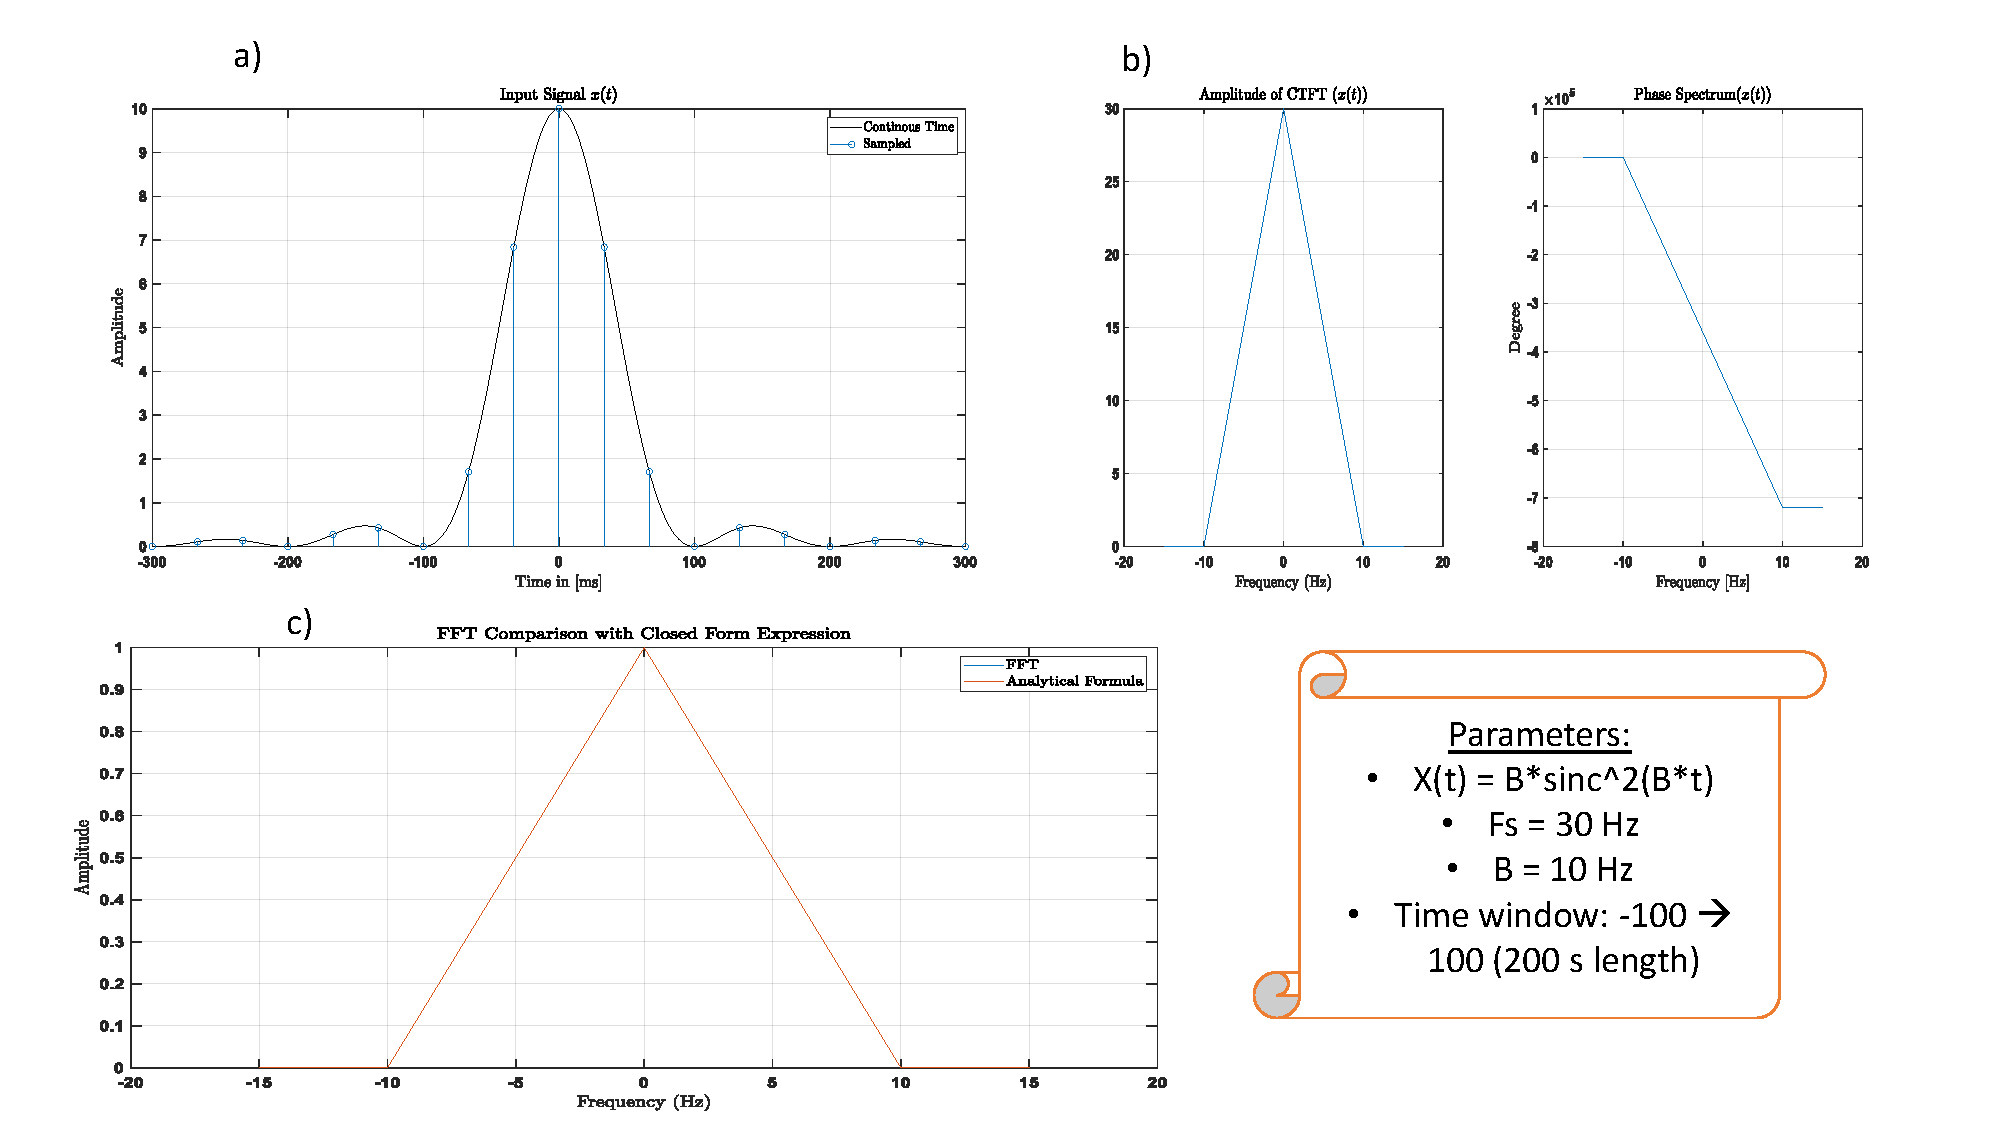
\includegraphics[scale = 0.5]{Figures/Sim_Fourier_Transform/sinc2_B_10Hz_Fs_30Hz}
\caption{Working with sinc square}
\label{fig:Sim_Fourier_Transform:sinc2_B_10Hz_Fs_30Hz}
\end{figure}

\begin{itemize}
    \item In order to obtain the unity amplitude in $\Delta\displaystyle \left( \, \frac{F}{2 \, B} \,\right)$, we need to divide by $F_s$ according to \autoref{Eq:DTFT-CTFT-Relation}.
\end{itemize}

\newpage
\subsection{Rect and Sinc Simulation}

Here are the result of some simulation for sinc and rect pulses presented in \autoref{fig:Sim_Fourier_Transform:res_sinc_rect_Fourier}


\begin{figure}[h]
\centering
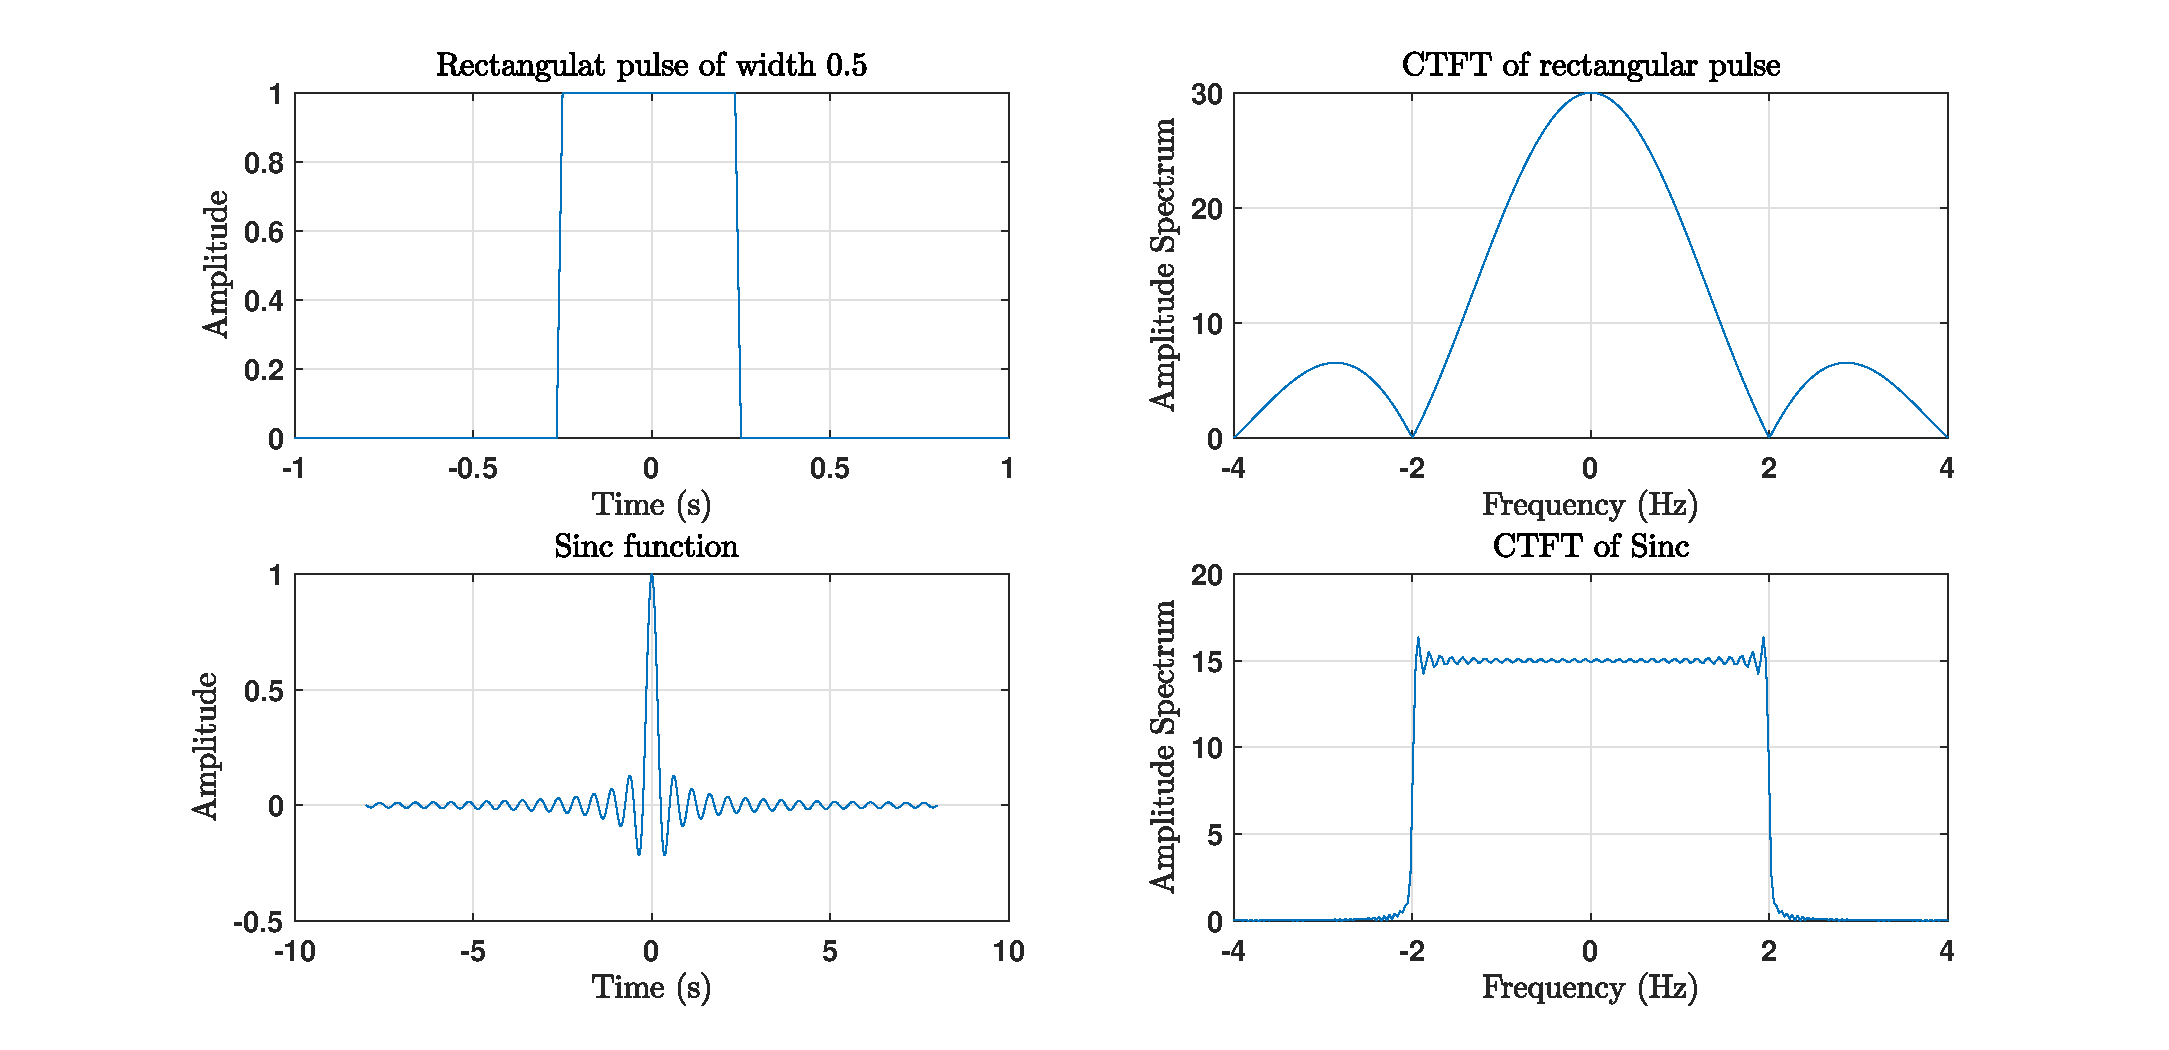
\includegraphics[scale = 0.5]{Figures/Sim_Fourier_Transform/res_sinc_rect_Fourier}
\caption{Plot of  $\text{rect} \left(\, \displaystyle\frac{t}{T} \, \right) \text{ and } \text{sinc}\left(\,  \displaystyle\frac{t}{T}  \, \right)$}
\label{fig:Sim_Fourier_Transform:res_sinc_rect_Fourier}
\end{figure}

\begin{itemize}
    \item $T$ is the pulse width for the sinc and rect
    
    \begin{itemize}
        \item for rect: the pulse width is divided in halfs before and after $t \, = \, 0$
        
        \item for sinc case: pulse wdith start from $t \, = \, 0$
        
    \end{itemize}
    
    \item Bandwidth:
    
    \begin{itemize}
        \item for rect: we have a null-to-null bandwdith equal ot $\displaystyle\frac{1}{T} \, = \, \displaystyle\frac{1}{0.5} \,  = \, 2$ Hz
        
        \item Same as for sinc: however the sinc is bandlimited unlike the rect: so after 2 Hz, we have 0 values for the amplitude spectrum
        
    \end{itemize}
    
\end{itemize}



\newpage

\section{IFFT}

\verb|ifft| command is used to take us back to the time domain given some discrete samples.\\

\underline{Note:} if the input of the \verb|ifft|,that is the complex vector (CTFT or DTFT) if shifted via \verb|fftshift| command, we need to undo it via \verb|ifftshift|.\\


\underline{Results:}

\begin{figure}[h]
\centering
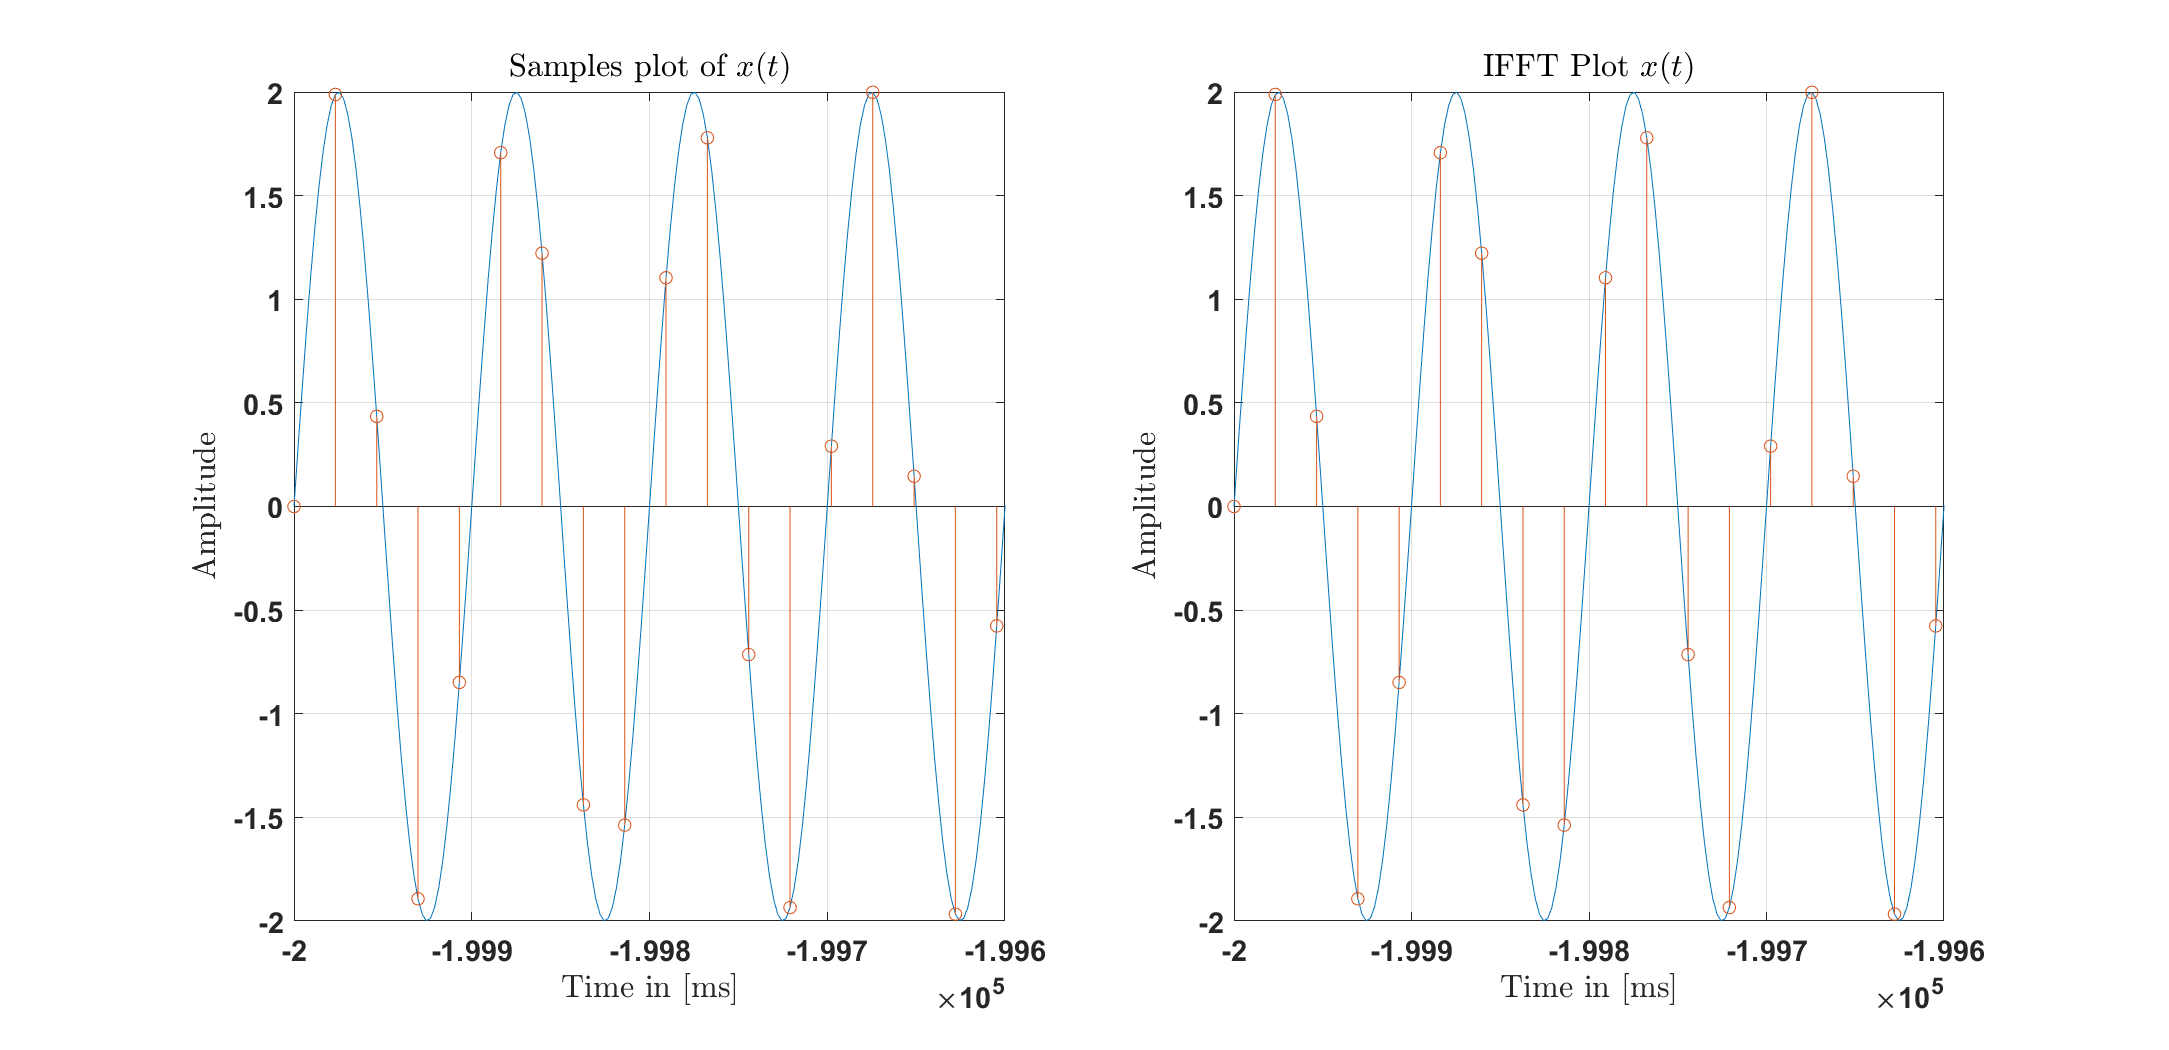
\includegraphics[scale = 0.25]{Figures/Sim_Fourier_Transform/ifft_sin_10_Hz}
\caption{Sin wave where $f \, = \, 10$ Hz}
\label{fig:Sim_Fourier_Transform:ifft_sin_10_Hz}
\end{figure}



\begin{figure}[h]
\centering
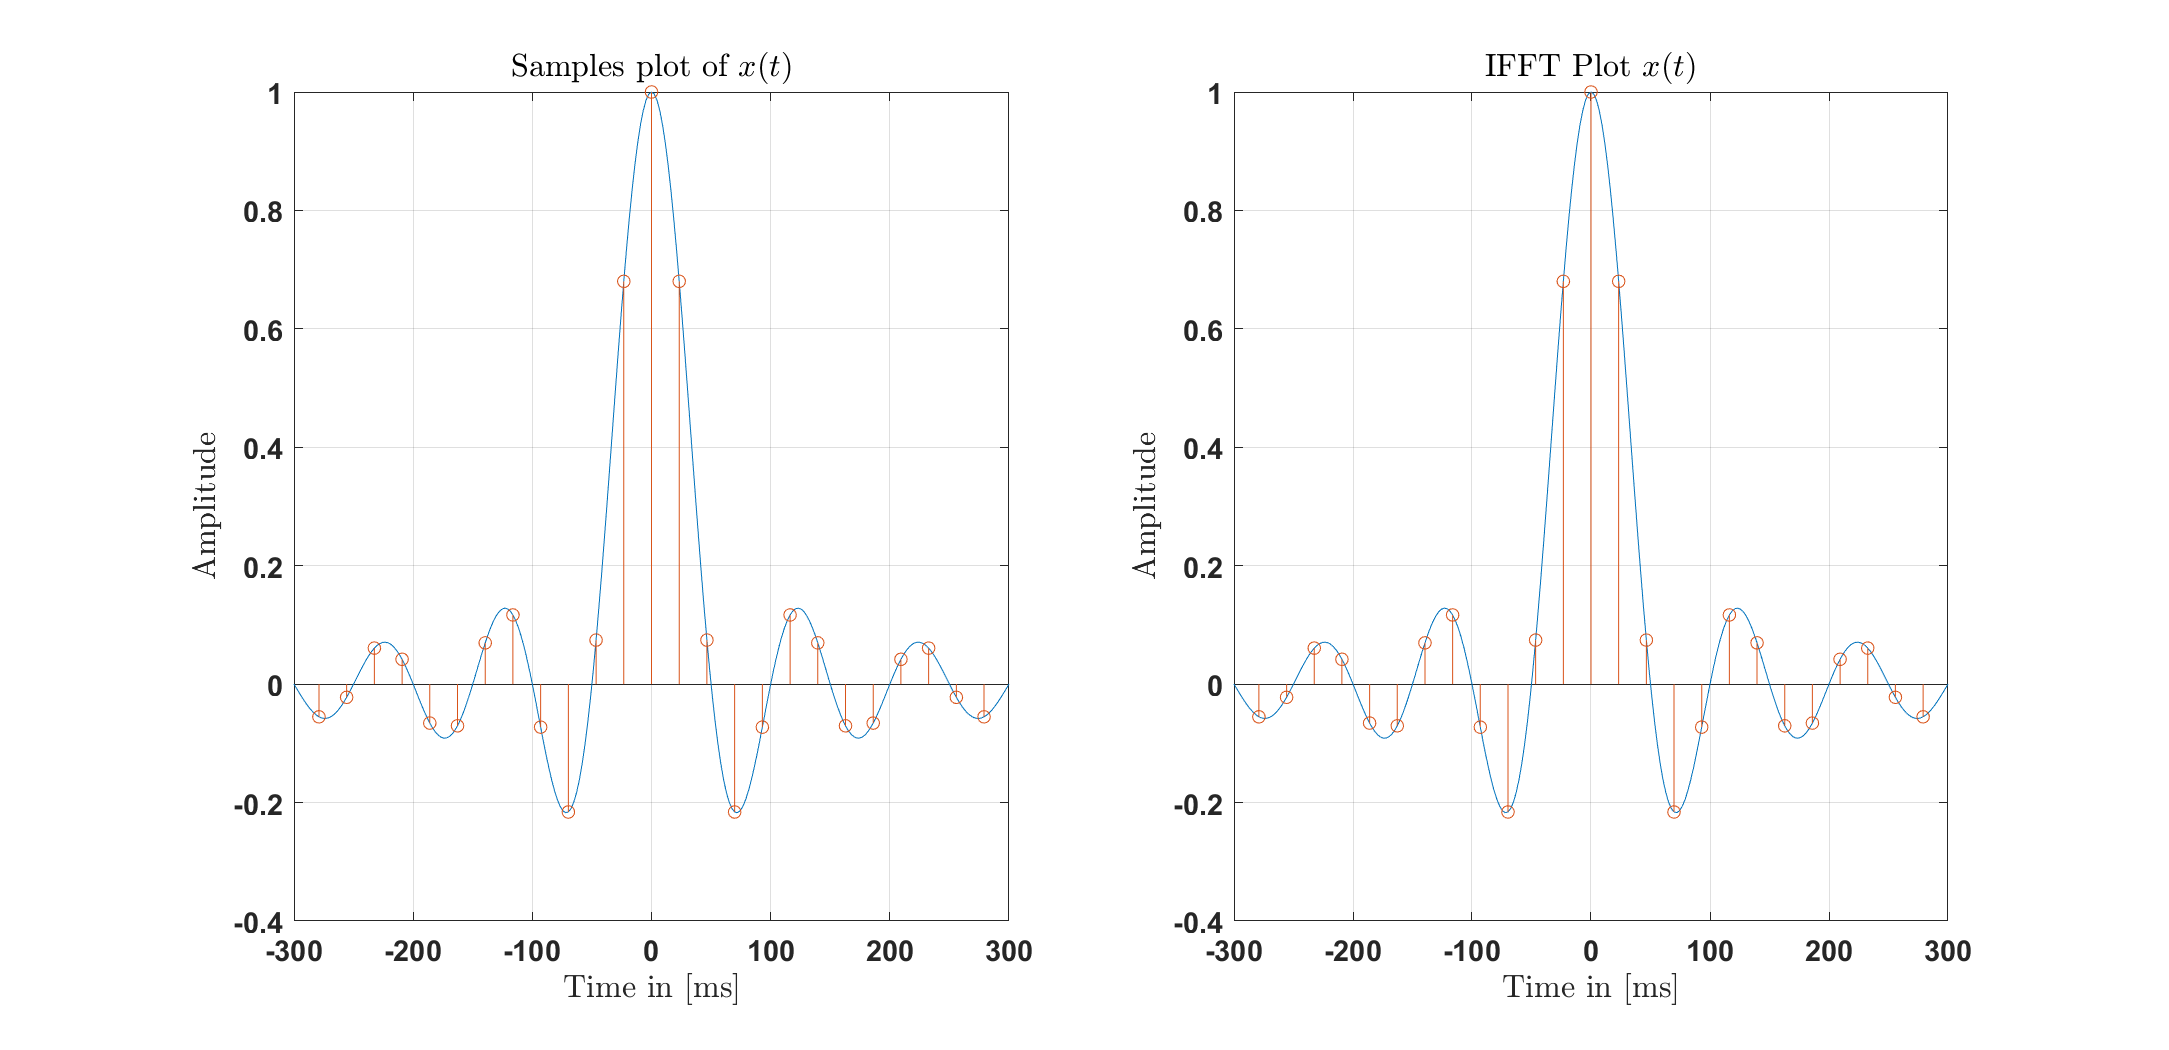
\includegraphics[scale = 0.25]{Figures/Sim_Fourier_Transform/ifft_rect_10_Hz}
\caption{Sinc wave where $B \, = \, 10$ Hz}
\label{fig:Sim_Fourier_Transform:ifft_rect_10_Hz}
\end{figure}

Even if we use zero padding in the \verb|fft|, in the \verb|ifft| we take a length equal to the number of samples (resulting from the uniform sampling process).



\newpage
\section{FFT over Multiple Period}

IN this section, we demonstrate how to plot an FFT spectrum over multiple period.

We all know that usually we plot the FFT from $\displaystyle\frac{-F_s}{2} \rightarrow \, \displaystyle\frac{F_s}{2}$. However, from sampling formula we know that a sampled spectrum is period over multiple of $F_s$.\\


What we can do to implement this periodicity of spectrum is to \tbi{set a new mapping} between the FFT index and the true frequency bin in Hz. This mapping is governed by the relation:


\begin{equation}
    f[\text{Hz}] \, = \, \overbrace{k}^{\text{freq index}}  \, \times \, \overbrace{\displaystyle\frac{F_s}{N}}^{\text{freq step}}
\end{equation}

such that $N \, = \, $ \verb|length-fft|.

A normal spectrum (from $0 \rightarrow F_s$, as the mathematics of DFT says) use the following values of $k$:

\begin{itemize}
    \item $k \, = \, 0 \rightarrow f[\text{Hz}] \, = \, 0$
    
    \item $k \, = \, N \, - \, 1 \rightarrow \, f[\text{Hz}] \, = \, \displaystyle\frac{N \, - \, 1}{N} \, \times \, F_s$
    
\end{itemize}

Then to generate a spectrum centered at 0, we use the \verb|fftshift| command, and the frequency axis using \verb|(-N/2:N/2 - 1) x Fs/N|.\\


Now suppose we want a spectrum from $\displaystyle\frac{-3\, F_s}{2} \rightarrow \, \displaystyle\frac{3 \, F_s}{2}$, the frequency bins generation will be \verb|(-3N/2:3N/2 - 1) x Fs/N|.

\newpage
An output of the simulation is shown in \autoref{fig:Sim_Fourier_Transform:Sinc_B_10Hz_Fs_30_Hz_Multiple_Period}

\begin{figure}[h]
\centering
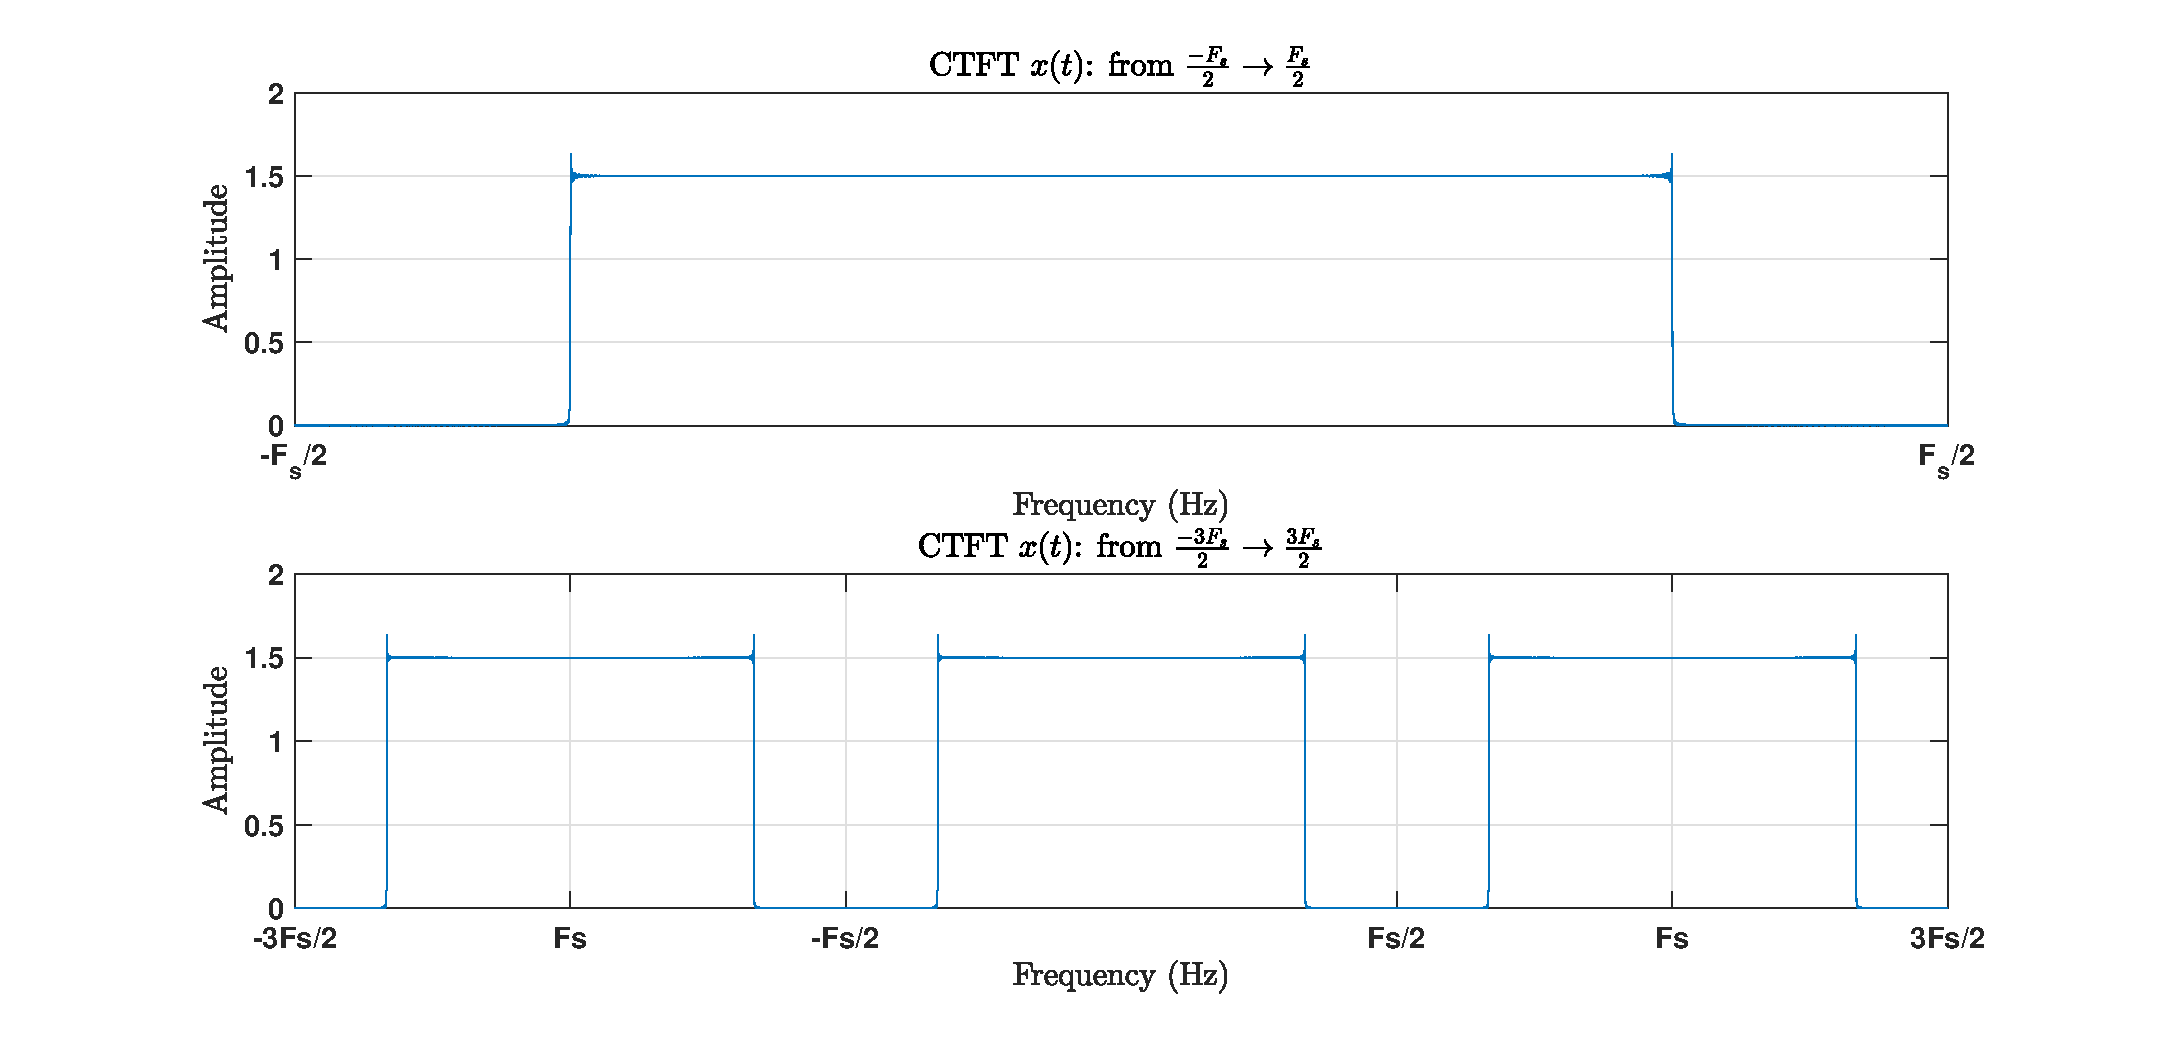
\includegraphics[scale = 0.5]{Figures/Sim_Fourier_Transform/Sinc_B_10Hz_Fs_30_Hz_Multiple_Period}
\caption{Sinc signal where $B \, = \, 10$ Hz and $F_s \, = \, 30$ Hz}
\label{fig:Sim_Fourier_Transform:Sinc_B_10Hz_Fs_30_Hz_Multiple_Period}
\end{figure}

\newpage
\section{Periodic Signals}

In previous section the work was focused on \textit{aperiodic continuous time signal}. Now we turn our attention to periodic signals.

We start with a square wave example, taken from \cite{paper_aliasing_matlab_Sol_Neeman}.

\begin{itemize}
    \item We take fundamental frequency $f_0 \, = \, 30$ Hz $\rightarrow T_0 \, = \, 0.033$s
    
    \item We set the duty cycle to 50 \% $\rightarrow$ in each period, the signal is 50 \% of the time up then down
    
    \item Sampling frequency is set to $F_s = 1$ KHz
    
\end{itemize}

\autoref{fig:Sim_Fourier_Transform:square_wave} shows result of simulation
 
\begin{figure}[h]
\centering
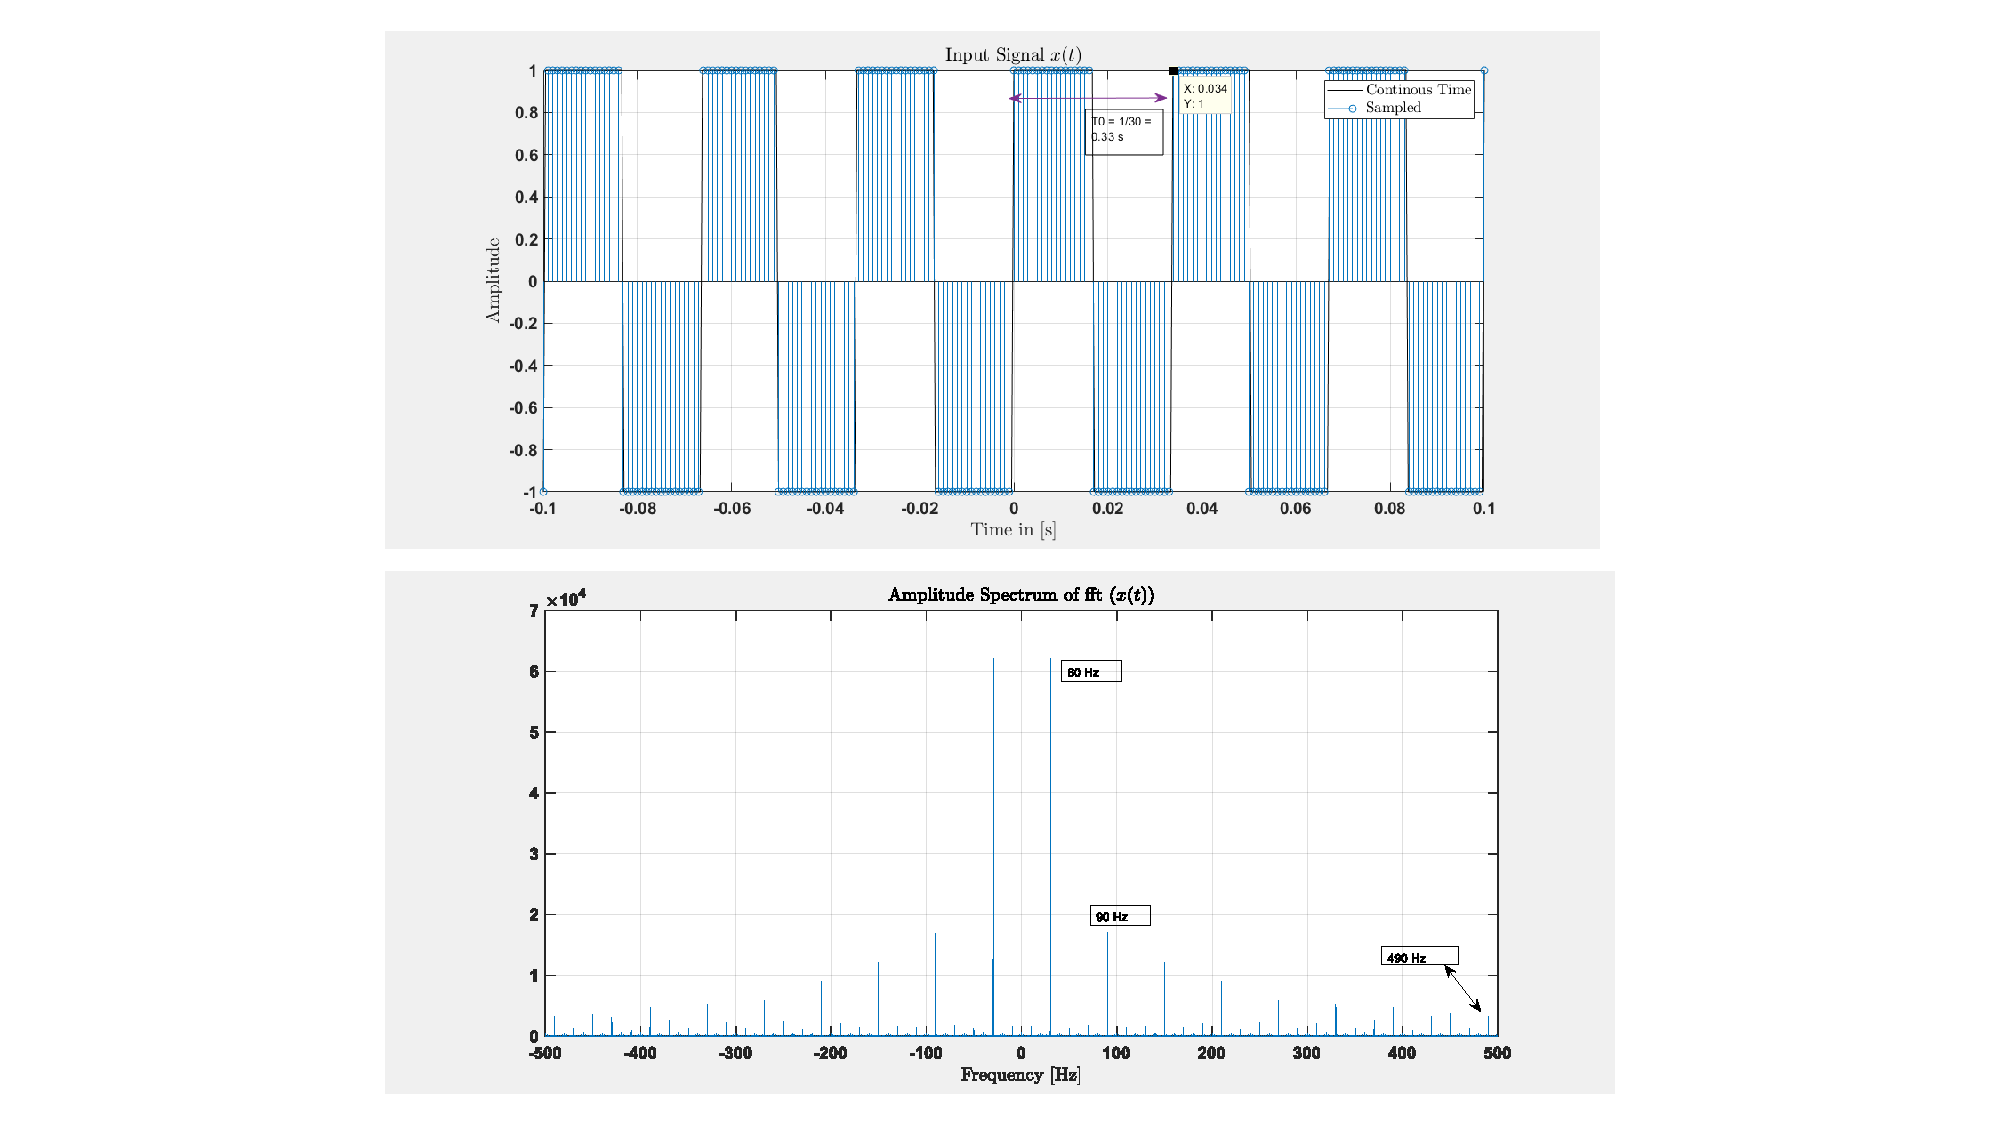
\includegraphics[scale = 0.5]{Figures/Sim_Fourier_Transform/Fourier_periodic_square_wave}
\caption{Square Wave with $F_0 \, = \, 30$ Hz}
\label{fig:Sim_Fourier_Transform:square_wave}
\end{figure}


\begin{itemize}
    \item Fourier Series expression: 
    
    \begin{equation}
        X(t) \, = \, \displaystyle\frac{4}{\pi} \displaystyle\sum_{k = 0}^\infty \displaystyle\frac{\text{sin}\left[ (2 k \, + \, 1) \, 2 \pi f_0 \, t \right]}{(2 k \, + \, 1)}
        \label{Eq:square_wave_fourier_series}
    \end{equation}
    
    
    \item Harmonics appear for odd nature
    
    \begin{itemize}
        \item $k = 0 \rightarrow \, (2k + 1) f_0 =  1 f_0 \, = \, 30$ Hz
        
        \item $k = 1 \rightarrow \, (2k + 1) f_0 =  3 f_0 \, = \, 90$ Hz
        
        \item $k = 2 \rightarrow \, (2k + 1) f_0 =  5 f_0 \, = \, 150$ Hz
        
    \end{itemize}
    
\end{itemize}

\subsection{Aliasing Effect}

It is important to note that the spectrum of doesn't only contains the harmonics, but also \tbi{aliased frequency components}.

Till now, we didn't treat the effect of aliasing in Fourier analysis, since we assume the sampling rate $F_s$ always bigger then the maximum frequency component $f_{\text{max}}$ in the spectrum $\rightarrow F_s > f_{\text{max}}$. (More  treatment to come about this topic in \autoref{Chap:Sampling_Reconstruction}).\\

Here in square wave signal, we don't have a $f_{\text{max}}$ (notice in \autoref{Eq:square_wave_fourier_series} the frequency component keep going to $\infty$). Since $F_s \, = \, 1$ KHz, every frequency component above $\displaystyle\frac{F_s}{2} = 500$ Hz will be aliased to the range of DC $\rightarrow \displaystyle\frac{F_s}{2} = 500$ Hz.

As example, 510 Hz ($k = 17$) will be aliased into 490 Hz as shown in the $\mathrm{2}^\mathrm{nd}$ row of \autoref{fig:Sim_Fourier_Transform:square_wave}.\\

\underline{Aliasing computation:} $490 = F_s \, - 510 = 490$


\newpage
\section{Signals used in Sampling}

\underline{Source:} See section 3.2.3 in \cite{sampling_beyond_band_limited_systems}.

\begin{itemize}
    \item $x(t) \, = \, \delta(t) \, \leftrightarrow \, X(\Omega) \, = \, 1$
    
    \begin{itemize}
        \item For a time shifted dirac: $x(t) \, = \, \delta(t \,- \, t_0) \leftrightarrow \, X(\Omega) \, = \, e^{j \, \Omega \, t_0}$
        
        
        \item Dual transform: 
        
        \begin{itemize}
            \item $x(t) \, = \, 1 \leftrightarrow \, X(\Omega) \, = \, 2 \pi \delta(\Omega)$: constant function (DC component) has its energy only at $\Omega \, = \, 0$ 
            
            \item $e^{j \Omega t_0} \leftrightarrow \, 2 \pi \, \delta(\Omega \, - \, \Omega_0)$: energy contained at $\Omega \, = \, \Omega_0$
            
        \end{itemize}

    \end{itemize}
    
\item Train of Dirac delta function: $x(t) \, = \, \displaystyle\sum\limits_{n \, \in \, \mathbb{Z}} \delta (t \,- \,  n \, T_s)$      


\newpage
\item Rectangular signal: $x(t) \, = \, \begin{cases}
1 \quad \displaystyle\frac{-1}{2} \, \leq t \, \, \leq \displaystyle\frac{1}{2} \\
0 \quad \text{otherwise}
\end{cases} \leftrightarrow \, X(\Omega) \, = \, \text{sinc}\left(\,  \displaystyle\frac{\Omega}{2 \pi}  \, \right)$

\begin{itemize}
    \item Dual transform and using time scale property: $\text{sinc}\left(\,  \displaystyle\frac{t}{T}  \, \right) \, \leftrightarrow \, X(\Omega) \, = \, T$ for $ \displaystyle\frac{-\pi}{T} \, \leq  \, \Omega \, \leq \,  \displaystyle\frac{\pi}{T}$ 
\end{itemize}

\begin{figure}[h]
\centering
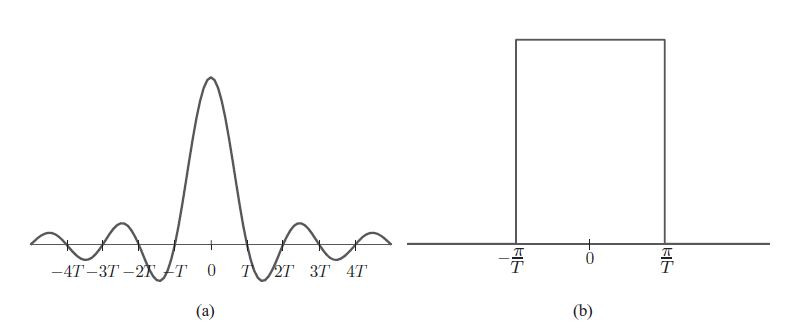
\includegraphics[scale = 0.5]{Figures/Sim_Fourier_Transform/sinc_rect_Fourier}
\caption{CTFT of $\text{sinc}\left(\,  \displaystyle\frac{t}{T}  \, \right)$ \cite{sampling_beyond_band_limited_systems}}
\label{fig:Sim_Fourier_Transform:sinc_rect_Fourier}
\end{figure}


\item Discrete Exponentials (section 3.3.2 in \cite{sampling_beyond_band_limited_systems}):

\begin{equation}
    x[n] \, = \, e^{j \, \omega_0 \, n} \leftrightarrow \, X(\omega) \, = \, 2 \pi \displaystyle\sum_{k \, \in \, \mathbb{Z}} \delta(\omega \, - \, \omega_0 \, + \, 2 \,  \pi \, k)
\end{equation}
    
\end{itemize}


\newpage
\section{Continuous–discrete Representations}

\underline{Source:} See section 3.2 in \cite{sampling_beyond_band_limited_systems}.\\

In context of sampling, we deals with a \tbi{mixed signal representation}, involving 2 components: a continuous time signal $x(t)$ and a discrete time sequence $d[n]$, having the form:


\begin{equation}
    x(t) \, = \, \displaystyle\sum_{n \in \mathbb{Z}} d[n] \, h(t \, - \, n \, T_s)
\end{equation}

Some facts:

\begin{itemize}
    \item $X(\Omega) \, = \, D(\omega) \, H(\Omega)$
\end{itemize}



%****************************************
%****************************************
%****************************************